\documentclass[11pt,letterpaper]{article}

% ============ DATOS DEL ESTUDIANTE ============
\newcommand{\nombreEstudiante}{Duván Felipe Baquero}
\newcommand{\codigoEstudiante}{160005002}
\newcommand{\nombreDocente}{Ángel Alfonso Cruz Roa}
% ==============================================

% Preámbulo agnóstico al motor: sirve con pdfLaTeX, XeLaTeX y LuaLaTeX.
\usepackage{iftex}
\ifPDFTeX
  \usepackage[utf8]{inputenc}
  \usepackage[T1]{fontenc}
  \usepackage{lmodern}
\else
  \usepackage{fontspec}
\fi

% babel-spanish redefine \% y rompe \,\% y el \% dentro de modo matemático.
\let\origpercent\%
\usepackage[spanish,es-tabla,es-nodecimaldot]{babel}
\AtBeginDocument{\let\%\origpercent}

\usepackage[margin=2.5cm]{geometry}
\usepackage{graphicx}
\usepackage{booktabs}
\usepackage{array}
\usepackage{amsmath}
\usepackage{amssymb}
\usepackage{float}
\usepackage{xcolor}
\usepackage{fancyhdr}
\usepackage{caption}
\usepackage{enumitem}
\usepackage{microtype}
\usepackage{tocloft}
\usepackage[hidelinks]{hyperref}

\setlength{\cftbeforesecskip}{0.45em}
\captionsetup{font=small,labelfont=bf,skip=6pt}
\setlength{\parskip}{0.35em}
\setlength{\emergencystretch}{3em}
\renewcommand{\arraystretch}{1.12}

% \input no es expandible y rompe \bottomrule dentro de tabular; se usa el primitivo
\makeatletter\newcommand{\tablain}[1]{\@@input #1 }\makeatother

\pagestyle{fancy}
\fancyhf{}
\lhead{\small Universidad de los Llanos}
\rhead{\small Simulación Computacional --- Laboratorio 5}
\rfoot{\small\thepage}
\renewcommand{\headrulewidth}{0.4pt}

\begin{document}

% =====================================================
% PORTADA
% =====================================================
\begin{titlepage}
\thispagestyle{empty}
\centering
\vspace*{\fill}

{\large \textsc{Universidad de los Llanos}}\\[0.2cm]
{\normalsize Facultad de Ciencias Básicas e Ingeniería}\\
{\normalsize Programa de Ingeniería de Sistemas}\\[1.6cm]

\rule{\textwidth}{0.8pt}\\[0.5cm]
{\LARGE \textbf{Análisis de datos de entrada y\\ bondad de ajuste}}\\[0.35cm]
{\large Estadística descriptiva, evaluación de independencia y\\
estabilidad, y ajuste de distribuciones de probabilidad}\\[0.5cm]
\rule{\textwidth}{0.8pt}\\[1.6cm]

{\normalsize Informe del Laboratorio 5}\\
{\normalsize (guía FO-DOC-112, Práctica N.\textsuperscript{o}\,04)}\\
{\normalsize Curso: Simulación Computacional}\\[1.4cm]

{\normalsize Presentado por:}\\[0.15cm]
{\large \nombreEstudiante}\\
{\normalsize Código: \codigoEstudiante}\\[1.2cm]

{\normalsize Docente:}\\[0.15cm]
{\large \nombreDocente}\\[1.6cm]

{\normalsize Villavicencio, Meta \\ \today}

\vspace*{\fill}
\end{titlepage}

\newpage
\tableofcontents
\newpage

% =====================================================
\section{Objetivos}
% =====================================================

Estos son los objetivos que trae la guía de laboratorio:

\begin{itemize}[itemsep=2pt]
    \item Introducir al análisis de datos de entrada en un estudio de simulación a partir de muestras de datos asociadas a procesos o fenomenos del sistema objeto de estudio.
    \item Identificar si un conjunto de valores de una muesta de datos asociados a algun proceso o fenomeno se puede asociar a una variable aleatoria independiente (no correlacionada), estacionaria.
    \item Evaluar la bondad de ajuste (godness of fit) de diferentes distribuciones de probabilidad a un conjunto de datos.
    \item Seleccionar la distribución de probabilidad más apropiada y con mejor ajuste dado un conjunto de datos para su posterior modelado en un estudio de simulación.
\end{itemize}

% =====================================================
\section{Consulta previa}
% =====================================================

\subsection{¿En qué consiste la estadística descriptiva?}

Es la parte de la estadística que resume un conjunto de datos sin intentar sacar conclusiones más allá de la
muestra. Lo hace con medidas numéricas y con gráficas. Las medidas son de tres tipos: de posición (media, mediana,
percentiles), de dispersión (rango, varianza, desviación estándar, coeficiente de variación) y de forma
(asimetría y curtosis). Las gráficas más comunes son el histograma, el diagrama de caja y la secuencia de valores.
En un estudio de simulación es el primer paso del análisis de datos de entrada, porque da una idea de qué familias
de distribuciones tiene sentido probar antes de hacer cualquier ajuste formal.

\subsection{¿Qué son la asimetría estadística (skewness), la curtosis y los percentiles?}

La asimetría mide qué tan desbalanceada está una distribución alrededor de su media. Se calcula como el tercer
momento estandarizado, $\gamma_1 = E[(X - \mu)^3]/\sigma^3$. Vale cero en una distribución simétrica como la normal;
es positiva cuando la cola larga está a la derecha (por ejemplo la exponencial, con $\gamma_1 = 2$) y negativa
cuando está a la izquierda. Un indicio práctico de asimetría positiva es que la media quede por encima de la mediana.

La curtosis es el cuarto momento estandarizado, $E[(X - \mu)^4]/\sigma^4$, y describe qué tan pesadas son las colas.
Se suele reportar en exceso respecto a la normal (restando 3), de modo que la normal tiene curtosis cero, una
distribución con colas más pesadas tiene curtosis positiva (la exponencial tiene 6) y una más achatada, negativa.

El percentil $p$ es el valor que deja por debajo al $p\,\%$ de los datos. Los más usados son los cuartiles:
$Q_1$ (25\,\%), $Q_2$ o mediana (50\,\%) y $Q_3$ (75\,\%). A diferencia de la media y la desviación estándar, no se
dejan arrastrar por valores extremos, lo que los hace útiles para describir datos muy sesgados.

\subsection{¿Qué significa el supuesto de que un conjunto de variables aleatorias sea IID?}

IID significa independientes e idénticamente distribuidas. Independientes quiere decir que el valor de una
observación no da información sobre las demás; idénticamente distribuidas, que todas salen de la misma
distribución, con los mismos parámetros, sin importar en qué momento se tomaron. Es el supuesto que hay detrás de
ajustar una sola distribución a una muestra y luego generar valores de ella en la simulación. Si falla la
independencia (los datos están correlacionados) o falla la idéntica distribución (el proceso cambia en el tiempo),
el modelo de entrada tiene que ser otro. Por eso, antes de ajustar, el capítulo 3 de \cite{banks98} pide revisar
los dos supuestos por separado.

\subsection{¿En qué consiste un proceso estocástico estacionario?}

Un proceso estocástico $\{X_t\}$ es una colección de variables aleatorias ordenadas en el tiempo. Es estacionario
(en sentido estricto) cuando su comportamiento probabilístico no cambia al desplazarse en el tiempo: la
distribución conjunta de $(X_{t_1}, \dots, X_{t_k})$ es la misma que la de $(X_{t_1+h}, \dots, X_{t_k+h})$ para
cualquier desplazamiento $h$. En la práctica se usa la estacionariedad débil, que pide que la media y la varianza
sean constantes y que la covarianza entre $X_t$ y $X_{t+h}$ dependa solo de la distancia $h$. Un proceso con
tendencia, como uno cuya media crece con el tiempo, no es estacionario. Para revisarlo se usan gráficas de la
secuencia, medias móviles y comparaciones entre tramos de la muestra.

\subsection{¿En qué consiste un proceso estocástico correlacionado?}

En uno en el que las observaciones cercanas en el tiempo están relacionadas entre sí, de modo que conocer un valor
ayuda a predecir el siguiente. La relación se mide con la autocorrelación de retraso $k$,
\[
\rho_k = \frac{\operatorname{Cov}(X_t, X_{t+k})}{\operatorname{Var}(X_t)},
\]
que en un proceso independiente vale cero para todo $k \ge 1$. Un ejemplo es el proceso autorregresivo de orden 1,
$X_t = \phi X_{t-1} + \varepsilon_t$, donde cada valor arrastra una parte del anterior y $\rho_k = \phi^k$. En
simulación es común en tiempos de servicio de operarios que se cansan o en tiempos de llegada que vienen en
rachas. Un proceso puede ser estacionario y correlacionado a la vez; la estacionariedad se refiere a que la
estructura no cambie en el tiempo, no a que los valores sean independientes.

% =====================================================
\section{Metodología y herramientas}
% =====================================================

El desarrollo está en dos cuadernos de Jupyter en Python, ejecutados de principio a fin. El ajuste de curvas va
en un cuaderno aparte porque la guía lo pide así:

\begin{center}
\begin{tabular}{@{}ll@{}}
\toprule
Numerales & Archivo \\
\midrule
5.1 y 5.2 & \texttt{Lab5\_5.1\_5.2\_\codigoEstudiante.ipynb} \\
5.3 & \texttt{Lab5\_5.3\_AjusteCurvas\_\codigoEstudiante.ipynb} \\
\bottomrule
\end{tabular}
\end{center}

Se usaron \texttt{numpy}, \texttt{pandas}, \texttt{matplotlib}, \texttt{scipy} y \texttt{statsmodels}, todas
disponibles en Google Colab. Los cuatro conjuntos (\texttt{dataset-A.txt} a \texttt{dataset-D.txt}) tienen 200
valores cada uno. Los cuadernos los leen de la misma carpeta o, si no están, los descargan de los enlaces de la
guía. Las gráficas del numeral 5.2 se hicieron con las funciones del cuaderno de ejemplo \emph{Example. Input Data
Analysis} y el ajuste del numeral 5.3 sigue el tutorial de \cite{amat2021} y los cuadernos de ejemplo del curso.

% =====================================================
\section{Numeral 5.1: estadística descriptiva}
% =====================================================

\subsection{Medidas estadísticas}

La tabla \ref{tab:51} reúne las medidas que pide la guía. La varianza y la desviación estándar son las
muestrales (con $n - 1$) y los percentiles se calcularon con interpolación lineal, que es el método por defecto de
\texttt{numpy}.

\begin{table}[H]
\centering
\caption{Descripción estadística de los conjuntos de datos A, B, C y D.}
\label{tab:51}
\small
\begin{tabular}{@{}lrrrr@{}}
\toprule
Medida estadística & Dataset A & Dataset B & Dataset C & Dataset D \\
\midrule
\tablain{tablas/tab51.tex}
\bottomrule
\end{tabular}
\end{table}

Como apoyo para leer la forma de cada distribución se calcularon también la asimetría, la curtosis en exceso, el
coeficiente de variación (desviación estándar sobre media) y el cociente entre media y mediana (tabla
\ref{tab:51forma}).

\begin{table}[H]
\centering
\caption{Medidas de forma.}
\label{tab:51forma}
\small
\begin{tabular}{@{}lrrrr@{}}
\toprule
Medida & Dataset A & Dataset B & Dataset C & Dataset D \\
\midrule
\tablain{tablas/tab51forma.tex}
\bottomrule
\end{tabular}
\end{table}

\begin{figure}[H]
\centering
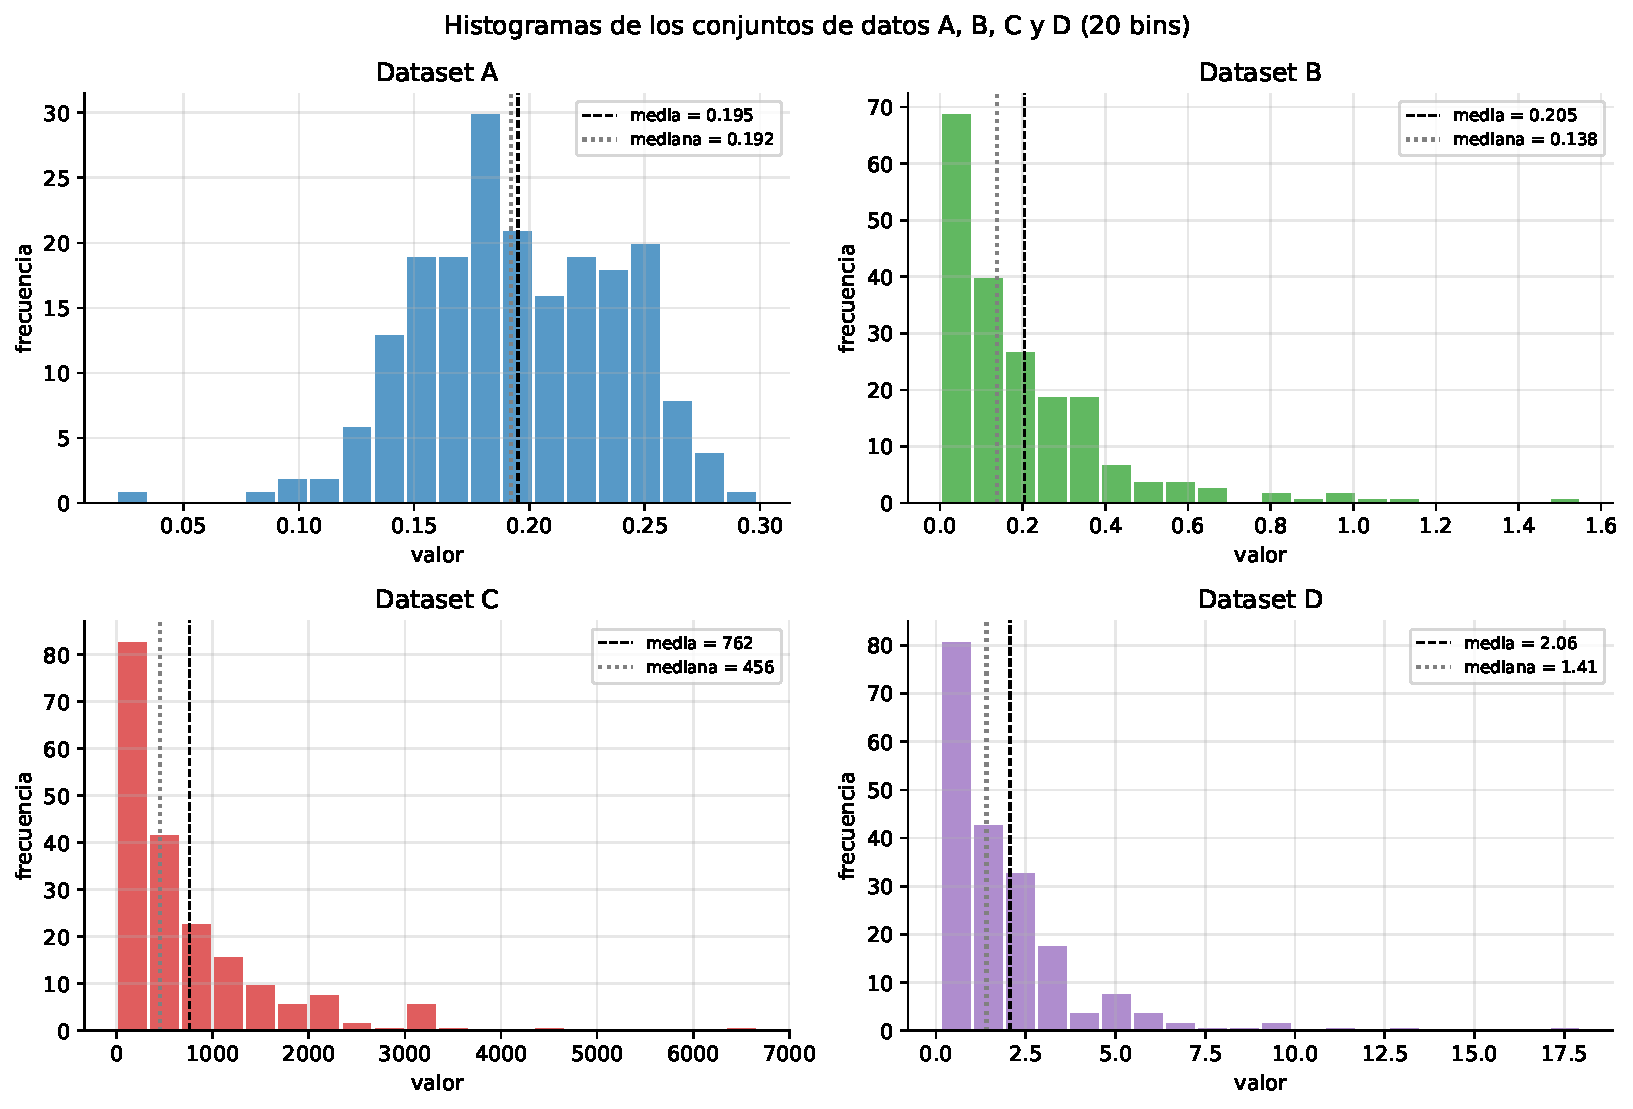
\includegraphics[width=0.92\textwidth]{figuras/51_histogramas.pdf}
\caption{Histogramas de distribuciones de los conjuntos de datos A, B, C y D (20 particiones). Las líneas
verticales marcan la media y la mediana.}
\label{fig:51}
\end{figure}

\subsection{¿Qué puede analizar de las medidas de estadística descriptiva y los histogramas?}

A primera vista los conjuntos forman dos grupos. A es el único con forma de campana: su media (0,1950) y su mediana
(0,1921) casi coinciden, la asimetría es leve y negativa ($-0{,}29$) y todos los valores caen en un rango corto,
de 0,021 a 0,299, con un coeficiente de variación de apenas 0,22. El valor 0,021 queda algo aislado, porque el
siguiente más pequeño es 0,081, y resulta ser el primero de la secuencia; en el numeral 5.2 se ve por qué. Con esa
forma acotada y casi simétrica, las candidatas naturales para A son la normal y la beta.

B, C y D tienen la forma típica de los tiempos entre llegadas: muchos valores pequeños y una cola larga a la
derecha. En los tres la media supera a la mediana entre un 47 y un 67\,\%, la asimetría pasa de 2,4 y el
coeficiente de variación está entre 1,12 y 1,21. Aun así hay diferencias. En B la media (0,2054) y la desviación
estándar (0,2291) son casi iguales, que es justo lo que pasa en una exponencial; su asimetría (2,41) y su curtosis
(7,97) también están cerca de los valores teóricos de esa distribución (2 y 6), y la barra más alta del histograma
está pegada al cero. D tiene una cola bastante más pesada, con asimetría de 3,16 y curtosis de 14,1, y su mínimo es
0,11, no cero; eso apunta más a una lognormal o una gamma que a una exponencial. C tiene una forma parecida a la de B
y D pero vive en otra escala: va de 0,93 a 6669,85, con media de 762,39 y varianza de 852\,169,66.

Un detalle llamativo es que A y B tienen media cercana a 0,2, igual que los conjuntos artificiales del cuaderno de
ejemplo del profesor, que simulan llegadas con tasa 5. Lo que ninguna de estas medidas puede decir es si los valores
son independientes o si el proceso cambia en el tiempo, porque tanto el histograma como los estadísticos ignoran el
orden en que llegaron los datos. Eso se revisa en el numeral siguiente.

% =====================================================
\section{Numeral 5.2: análisis de datos de entrada}
% =====================================================

\subsection{Procedimiento}

Se usaron las funciones del cuaderno de ejemplo, que interpretan cada valor como un tiempo entre llegadas: la suma
acumulada da los instantes de llegada, con los que se construyen el patrón de hora de llegada y el conteo por
intervalos. Al adaptarlas a estos datos se hicieron cuatro cambios:

\begin{enumerate}[itemsep=2pt]
\item El ejemplo fija el horizonte en $T = 200$ porque sus datos artificiales se generaron en 200 unidades de
tiempo. Aquí ese horizonte no se conoce, así que se tomó como la suma de los 200 valores, que es el instante de la
última llegada.
\item En \texttt{plotArrivalCountsIntervals} el conteo del intervalo $k$ se guardaba en \texttt{counts[k-1]}, de
modo que el primer intervalo terminaba dibujado en la última barra. Se corrigió el índice y el conteo se hizo con
\texttt{np.histogram}, que además incluye los bordes de cada intervalo.
\item La media móvil del ejemplo usa una ventana de 100 observaciones, pensada para series de unas 1000 llegadas.
Con 200 datos esa ventana promedia la mitad de la muestra a la vez y aplana cualquier cambio, por lo que se usó una
ventana de 20.
\item Las cinco gráficas de cada conjunto se juntaron en una sola figura, junto con la secuencia de valores.
\end{enumerate}

Para no depender solo de la lectura visual se calcularon tres indicadores: la autocorrelación de retraso 1 con su
banda del 95\,\% ($\pm 1{,}96/\sqrt{n} = \pm 0{,}139$), la prueba de Ljung-Box con 10 retrasos, cuya hipótesis nula
es que no hay autocorrelación, y la correlación de Spearman entre cada valor y su posición en la secuencia, que
detecta tendencias.

\subsection{Gráficas}

\begin{figure}[H]
\centering
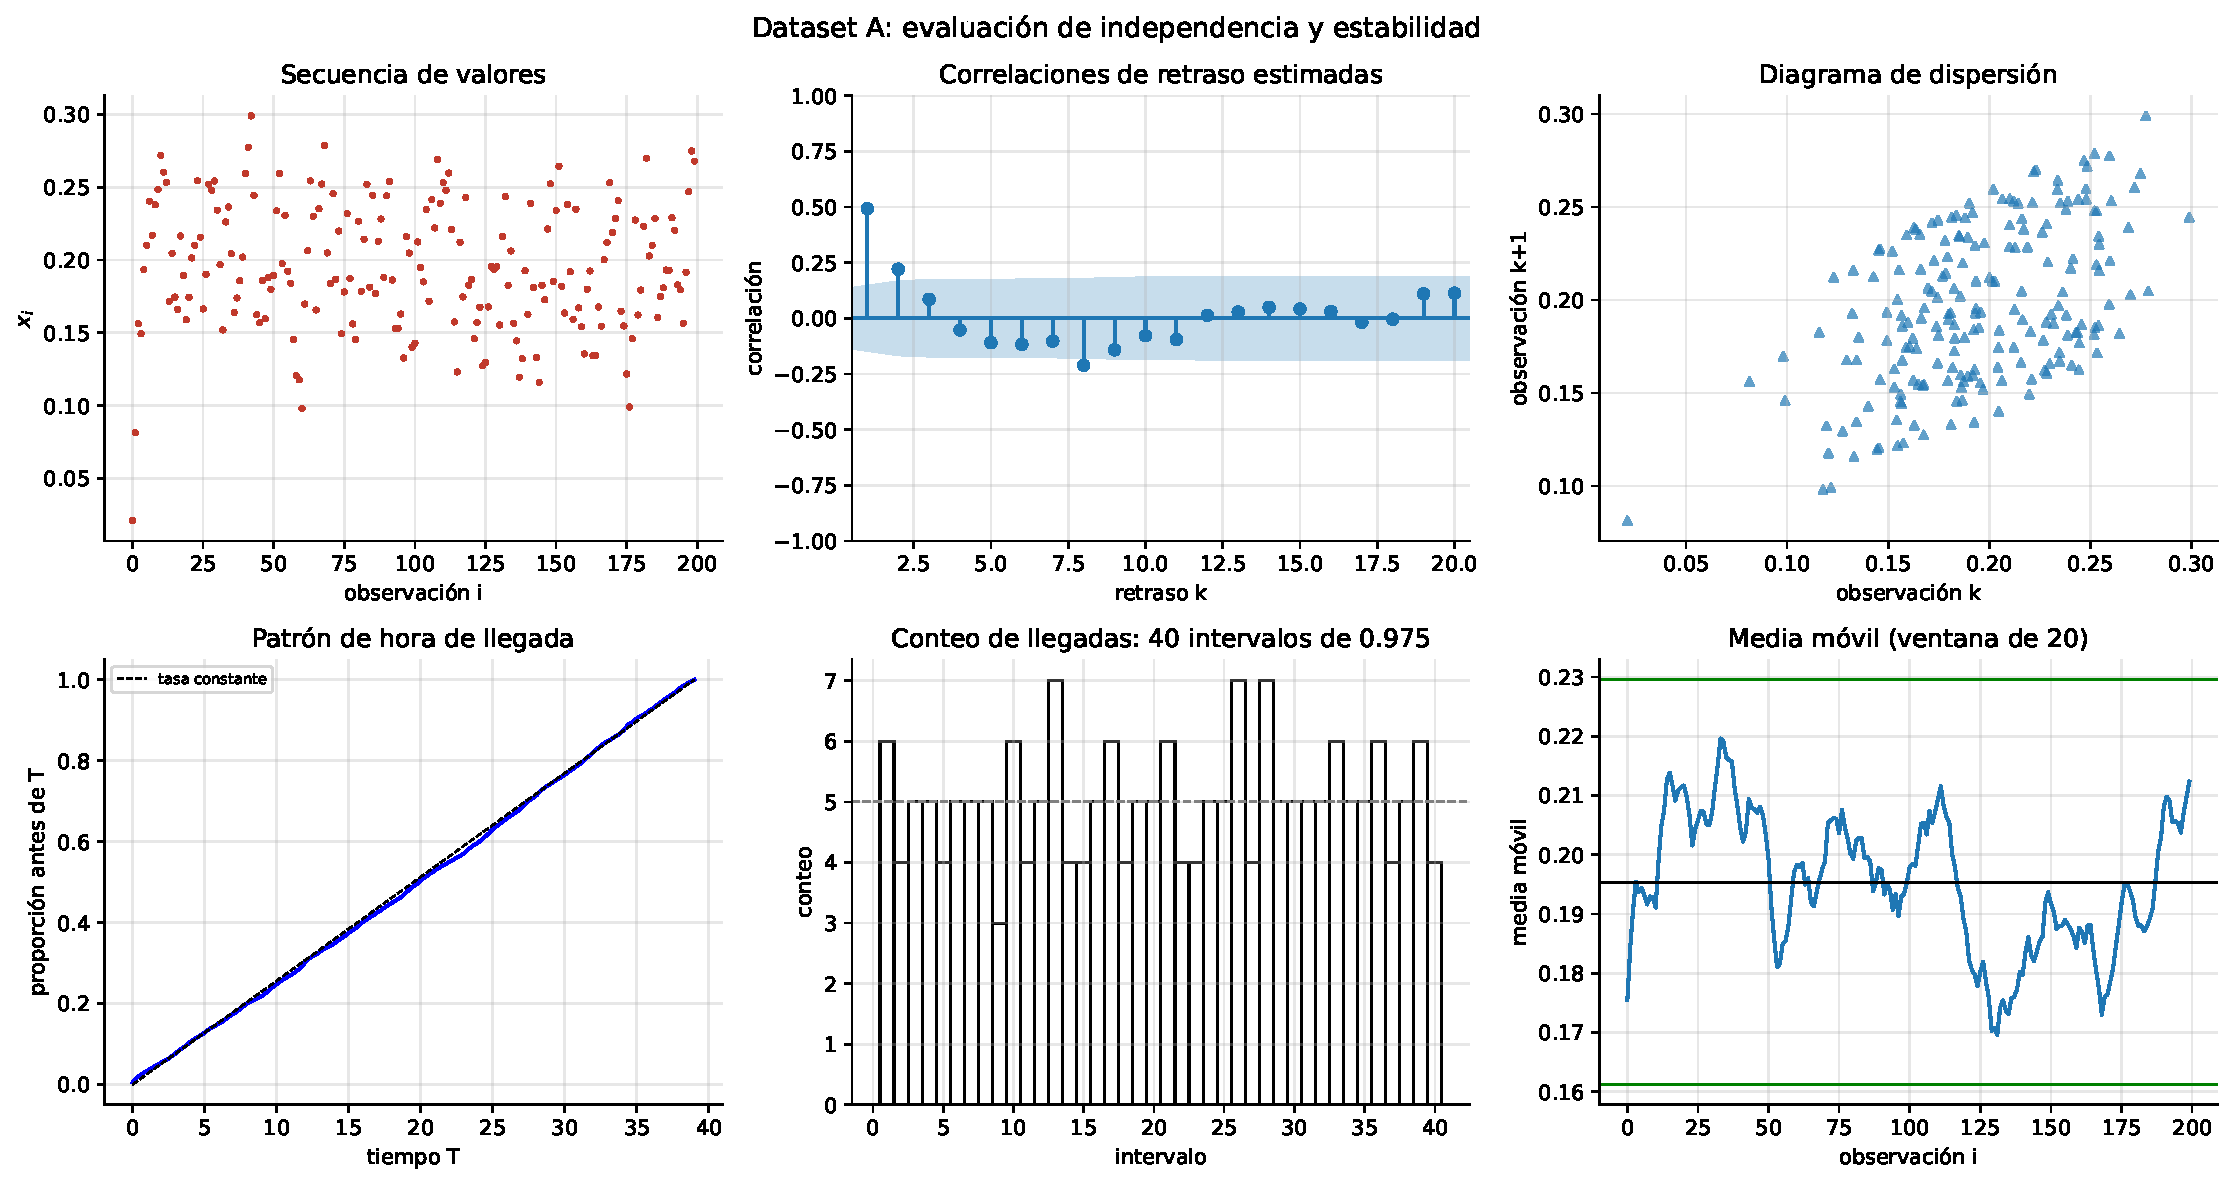
\includegraphics[width=\textwidth]{figuras/52_datasetA.pdf}
\caption{Dataset A: secuencia de valores, correlaciones de retraso estimadas, diagrama de dispersión, patrón de
hora de llegada, conteo de llegadas por intervalos y media móvil.}
\label{fig:52A}
\end{figure}

\begin{figure}[H]
\centering
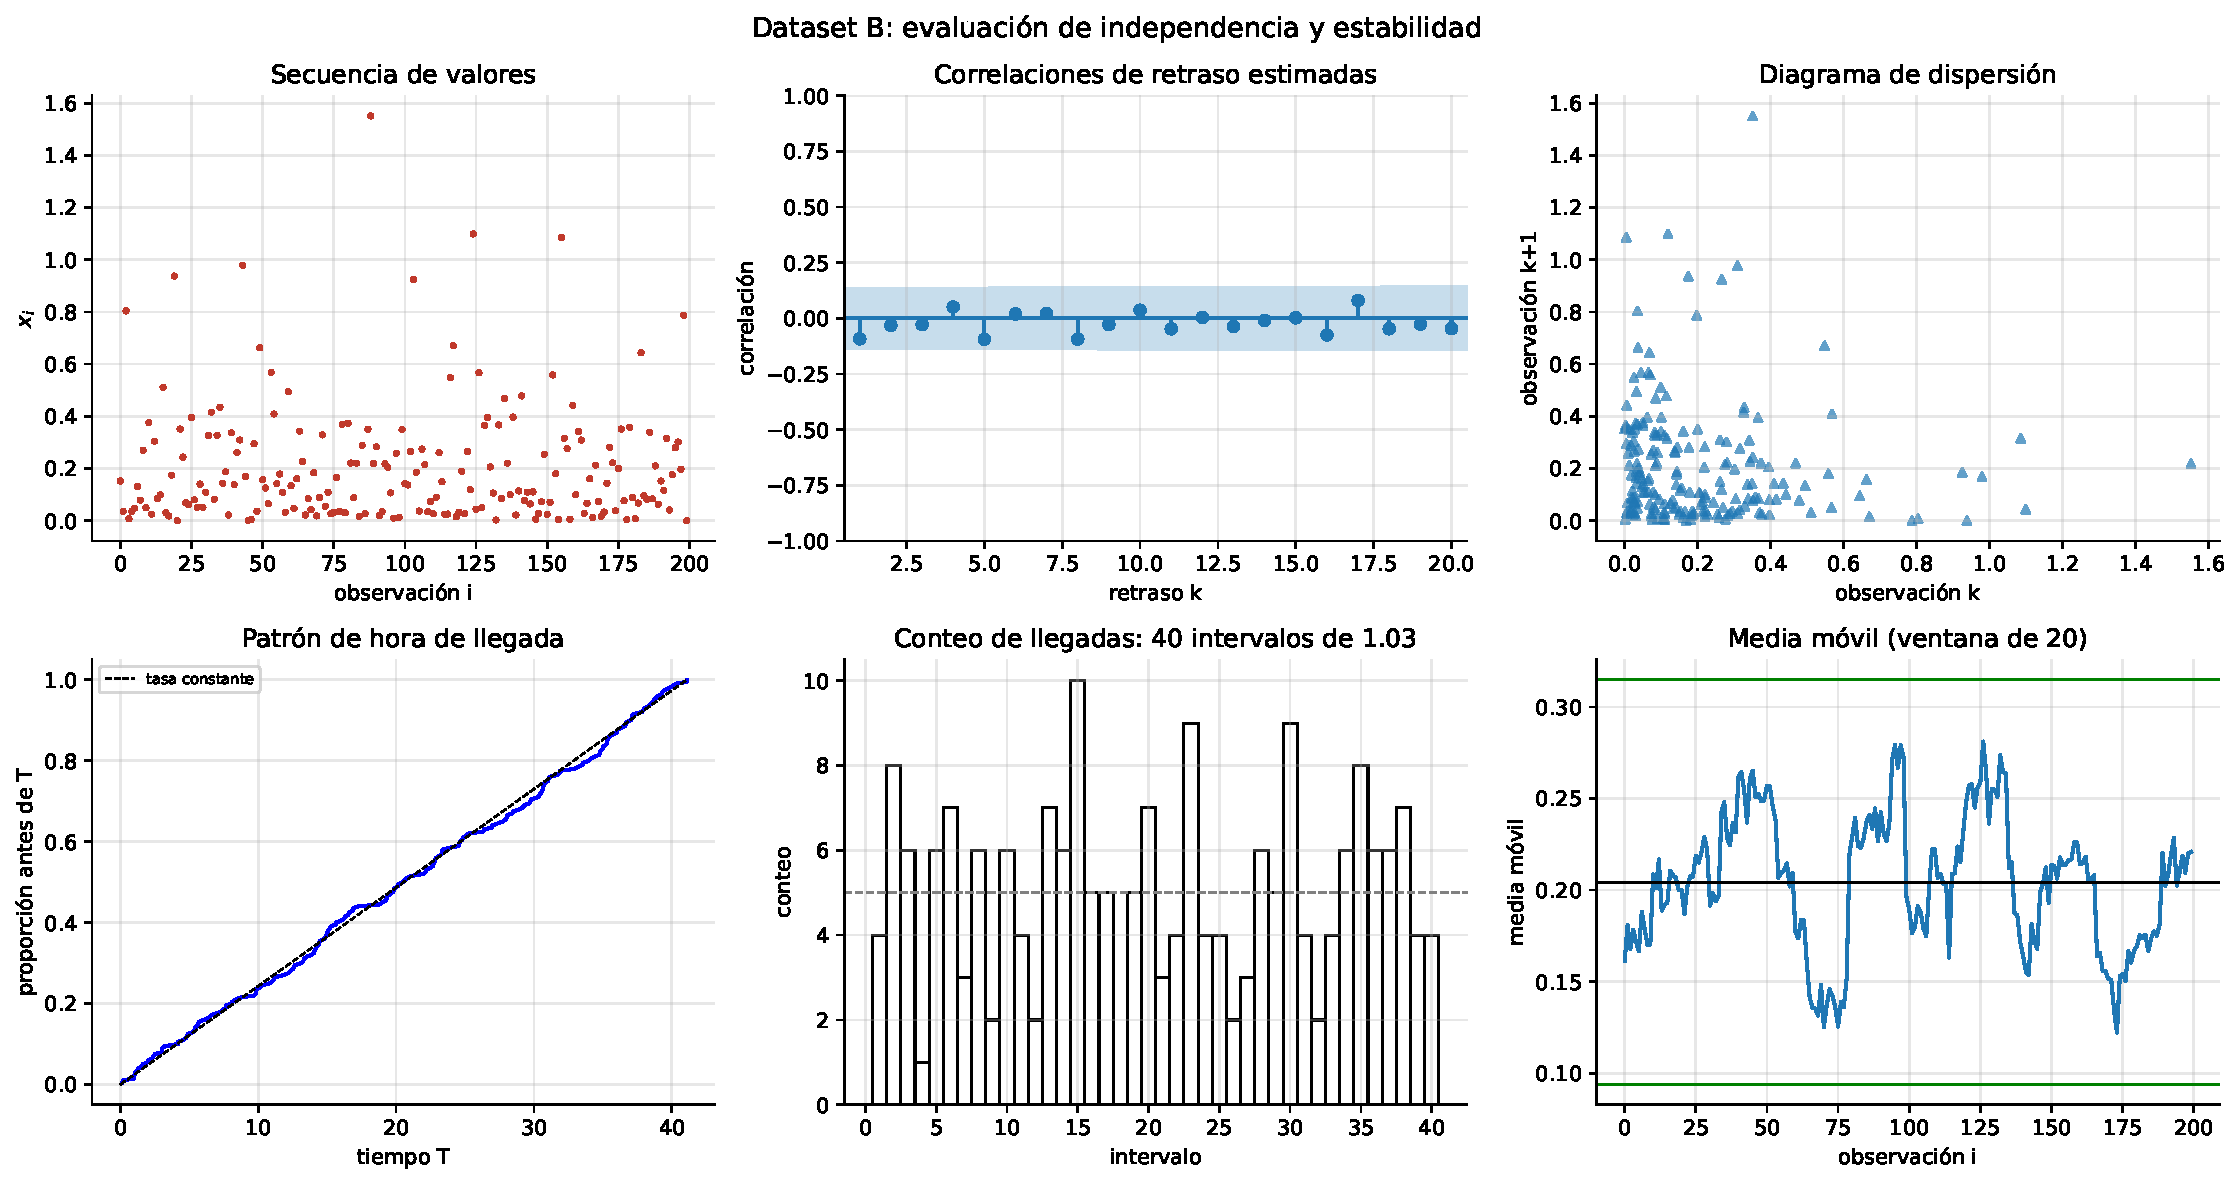
\includegraphics[width=\textwidth]{figuras/52_datasetB.pdf}
\caption{Dataset B: las mismas seis gráficas.}
\label{fig:52B}
\end{figure}

\begin{figure}[H]
\centering
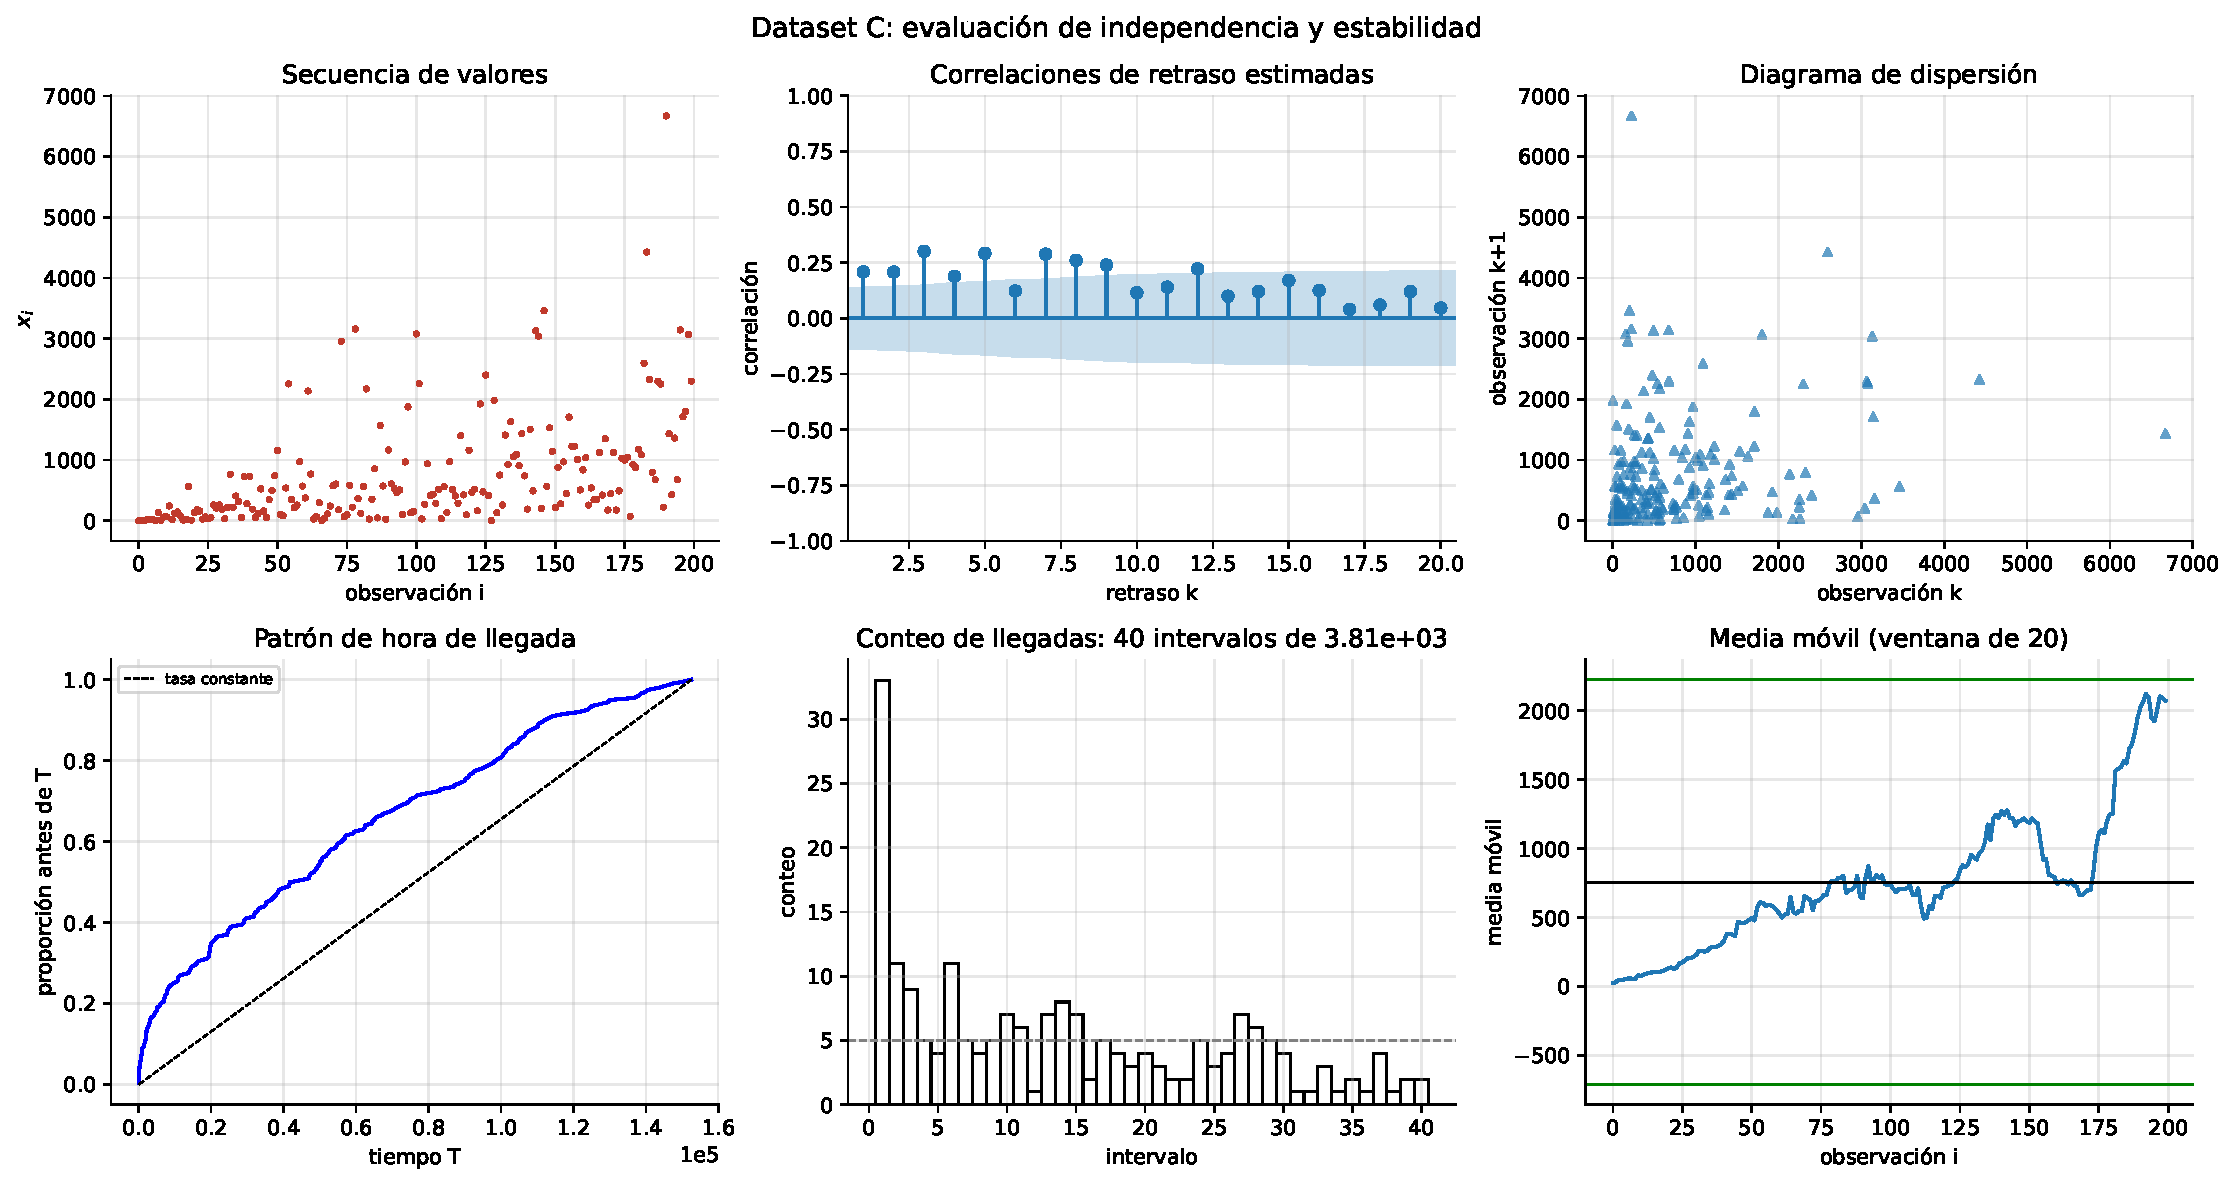
\includegraphics[width=\textwidth]{figuras/52_datasetC.pdf}
\caption{Dataset C: las mismas seis gráficas.}
\label{fig:52C}
\end{figure}

\begin{figure}[H]
\centering
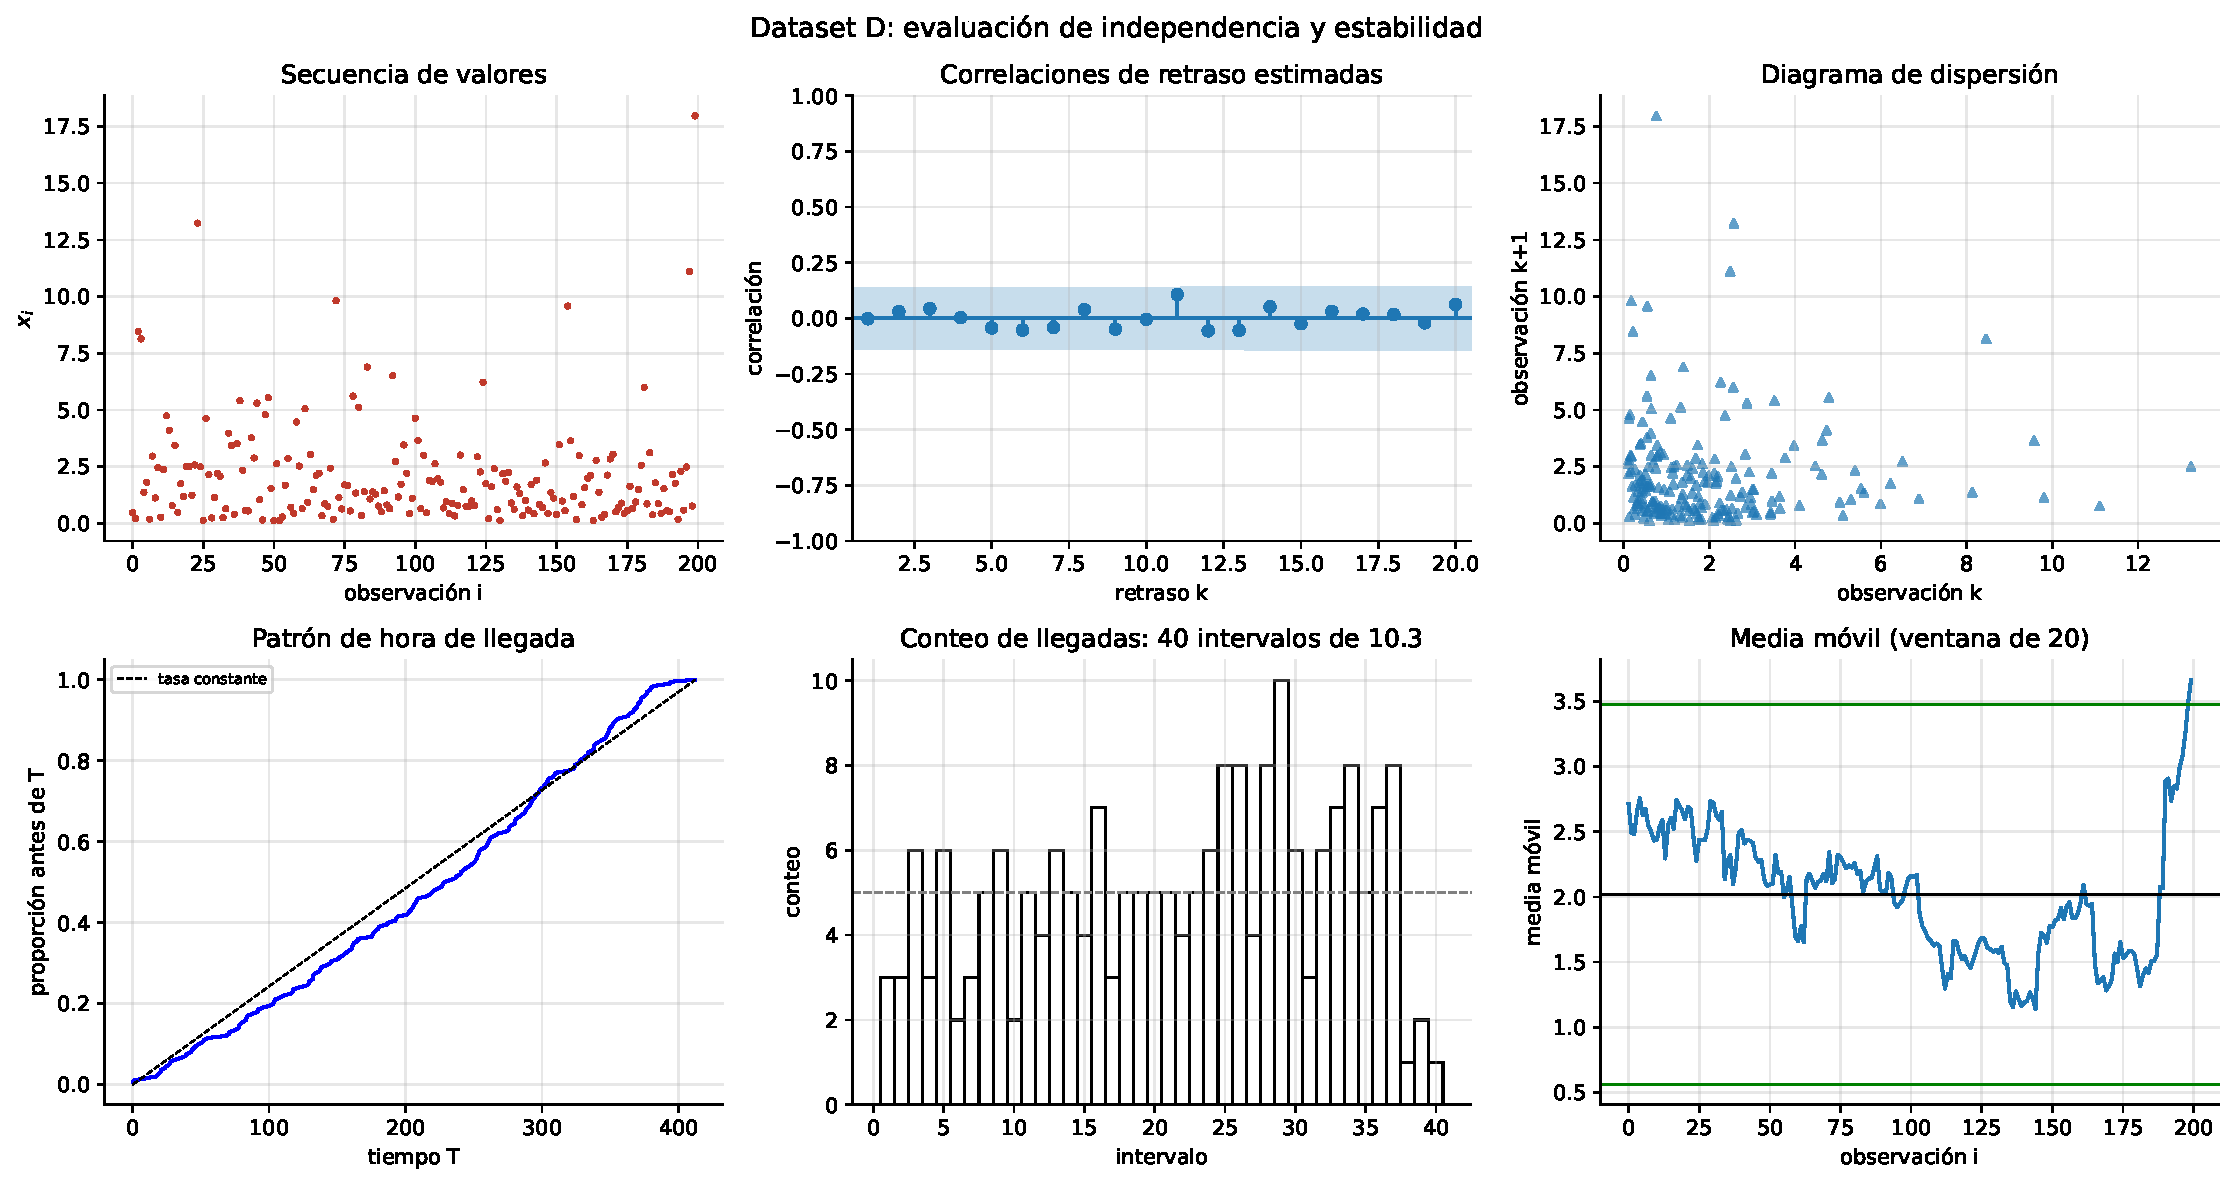
\includegraphics[width=\textwidth]{figuras/52_datasetD.pdf}
\caption{Dataset D: las mismas seis gráficas.}
\label{fig:52D}
\end{figure}

\begin{table}[H]
\centering
\caption{Indicadores de independencia y estabilidad.}
\label{tab:52ind}
\small
\begin{tabular}{@{}lrrrr@{}}
\toprule
Indicador & Dataset A & Dataset B & Dataset C & Dataset D \\
\midrule
\tablain{tablas/tab52ind.tex}
\bottomrule
\end{tabular}
\end{table}

\begin{table}[H]
\centering
\caption{Media de cada quinto de la secuencia (40 observaciones por tramo).}
\label{tab:52q}
\small
\begin{tabular}{@{}lrrrr@{}}
\toprule
Tramo & Dataset A & Dataset B & Dataset C & Dataset D \\
\midrule
\tablain{tablas/tab52quintos.tex}
\bottomrule
\end{tabular}
\end{table}

\subsection{¿Qué se puede determinar de cada conjunto sobre independencia y estabilidad?}

\subsubsection*{Dataset A: estacionario pero correlacionado}

La correlación de retraso 1 es 0,49, más de tres veces la banda del 95\,\%, y la de retraso 2 (0,22) también se sale
de ella; la prueba de Ljung-Box rechaza la independencia con $p < 0{,}0001$. En el diagrama de dispersión la nube
sube en diagonal: a un valor alto le suele seguir otro alto. En cambio, no se ven señales de inestabilidad. Las
medias por quintos van de 0,181 a 0,203, la correlación con la posición no es significativa ($p = 0{,}14$), el patrón
de llegadas va pegado a la diagonal de tasa constante y los conteos por intervalo oscilan alrededor de 5. Es el mismo
comportamiento del conjunto 6 del cuaderno de ejemplo, en el que cada valor es una combinación del anterior y de un
número uniforme. Eso también explica el valor aislado de 0,021 que se vio en el numeral 5.1: es el valor inicial de
la serie y no sale de la recurrencia. Para simular este proceso no basta con ajustar una distribución y sacar valores
independientes; habría que reproducir la dependencia.

\subsubsection*{Dataset B: compatible con IID}

Todas las correlaciones de retraso quedan dentro de la banda (la de retraso 1 es $-0{,}09$), Ljung-Box da
$p = 0{,}73$ y el diagrama de dispersión no muestra ningún patrón, solo la acumulación de puntos cerca del origen que
se espera de una exponencial. La correlación con la posición es prácticamente cero ($p = 0{,}96$), el patrón de
llegadas es una línea recta y los conteos fluctúan entre 0 y 10 alrededor de 5, como en un proceso de Poisson. La
media móvil sube y baja, pero nunca se sale de los límites de tres desviaciones. B es el candidato más claro para
ajustarle una sola distribución.

\subsubsection*{Dataset C: no estacionario}

Es el caso más claro de los cuatro. Las medias por quintos pasan de 153 a 570, 676, 1060 y 1352, es decir, la media
se multiplica casi por nueve entre el comienzo y el final, y la correlación de Spearman con la posición es de 0,60
con $p \approx 3 \times 10^{-21}$. La media móvil sube de forma sostenida y el patrón de llegadas queda muy por
encima de la diagonal: vistos como tiempos entre llegadas, los valores crecen y las llegadas se van espaciando. Por
eso 33 de los 200 eventos caen en el primero de los 40 intervalos, cuando lo esperado sería 5, y solo 2 en el
último. Las correlaciones son positivas en todos los retrasos (entre 0,1 y 0,3) y Ljung-Box también rechaza la
independencia, pero esa correlación viene en buena parte de la tendencia: dos valores cercanos se parecen porque
comparten el mismo nivel. Ajustar una sola distribución a C mezclaría niveles muy distintos. Según la sección 3.6 de
\cite{banks98}, en un caso no IID como este hay que modelar la tendencia, por ejemplo con un parámetro que cambie con
el tiempo.

\subsubsection*{Dataset D: compatible con IID, con una salvedad}

Las correlaciones están todas dentro de la banda ($r_1 = -0{,}002$) y Ljung-Box da $p = 0{,}99$, así que no hay
evidencia de dependencia. La estabilidad es menos limpia que en B: las medias por quintos bajan de 2,58 a 1,68 y
luego suben a 2,10, el patrón de llegadas queda un poco por debajo de la diagonal en la parte media y la correlación
con la posición es $-0{,}12$, aunque con $p = 0{,}099$ no alcanza a ser significativa al 5\,\%. El salto de la media
móvil al final se debe a que los dos últimos valores son 11,11 y 17,97 (este último es el máximo de toda la muestra)
y en el borde la ventana solo alcanza a promediar 10 datos. Con una cola tan pesada estas variaciones son
esperables, así que D se puede tratar como IID, aunque con más datos convendría volver a revisar la estabilidad.

\subsubsection*{Conclusión del numeral}

B y D cumplen el supuesto IID y se les puede ajustar una distribución directamente. A es estacionario pero
dependiente, y C no es estacionario. En el numeral 5.3 se ajustan las distribuciones a los cuatro conjuntos, como
pide la guía, pero para A y C la distribución ajustada solo describe la forma global de los datos y no alcanza para
simular el proceso.

% =====================================================
\section{Numeral 5.3: ajuste de curvas}
% =====================================================

\subsection{Distribuciones ajustadas}

La guía enumera cinco distribuciones obligatorias (exponencial, lognormal, normal, gamma y beta), aunque en el texto
dice ``cuatro'', y pide otras cuatro de libre elección; la tabla de ejemplo tiene, en efecto, nueve filas. Además de
las cinco se ajustaron:

\begin{itemize}[itemsep=1pt]
\item la Weibull, muy usada para tiempos de vida y de servicio, que incluye a la exponencial como caso particular;
\item la log-logística, de cola pesada, parecida a la lognormal pero con acumulada en forma cerrada;
\item la gaussiana inversa, otra alternativa para tiempos positivos y sesgados;
\item la triangular, la distribución que se suele usar en simulación cuando hay pocos datos y que podía servir para
la forma acotada de A.
\end{itemize}

Todas se ajustaron por máxima verosimilitud con \texttt{scipy.stats}. Como B, C y D son tiempos positivos, las
distribuciones definidas en $(0, \infty)$ se ajustaron con localización fija en cero, para trabajar con su forma de
dos parámetros (uno en la exponencial), que es la que se usa en simulación. La beta y la triangular necesitan un
intervalo $[a, b]$, que se estimó con el mínimo y el máximo de la muestra ampliados un poco:
$a = \max(0,\ x_{(1)} - r/(n-1))$ y $b = x_{(n)} + r/(n-1)$, con $r$ el rango.

\subsection{Criterios de bondad de ajuste}

Si $n$ es el tamaño de la muestra, $k$ el número de parámetros estimados con los datos y $\hat{L}$ la verosimilitud
máxima del modelo:
\[
\mathrm{SSE} = \sum_{j=1}^{20}\big(h_j - \hat{f}(c_j)\big)^2, \qquad
\mathrm{AIC} = 2k - 2\ln\hat{L}, \qquad
\mathrm{BIC} = k\ln n - 2\ln\hat{L},
\]
donde $h_j$ es la altura del histograma normalizado en la clase $j$ y $c_j$ su centro. En los tres casos, menor es
mejor. El SSE se calculó con las mismas 20 clases del numeral 5.1 y evaluando la densidad en los centros de las
clases, como en el cuaderno \emph{Fitting Niño data to a distribution}. No se siguió el cuaderno \emph{Fitting data
to a distribution}, porque allí la densidad se evalúa en \texttt{np.linspace(0, 100, 100)} y se compara con 100
barras del histograma que no están en esos mismos puntos.

Para escoger las tres mejores distribuciones de cada conjunto se ordenaron por cada criterio y se promediaron los
tres rangos; en caso de empate decide el AIC. En las tablas siguientes el superíndice indica ese orden y en negrita
está el mejor valor de cada criterio.

\subsection{Dataset A}

\begin{table}[H]
\centering
\caption{Bondad de ajuste para el conjunto de datos A.}
\label{tab:53A}
\footnotesize\setlength{\tabcolsep}{4pt}
\begin{tabular}{@{}l>{\raggedright\arraybackslash}p{6.4cm}rrr@{}}
\toprule
Distribución & Parámetros & SSE & AIC & BIC \\
\midrule
\tablain{tablas/tab53_A.tex}
\bottomrule
\end{tabular}
\end{table}

\begin{figure}[H]
\centering
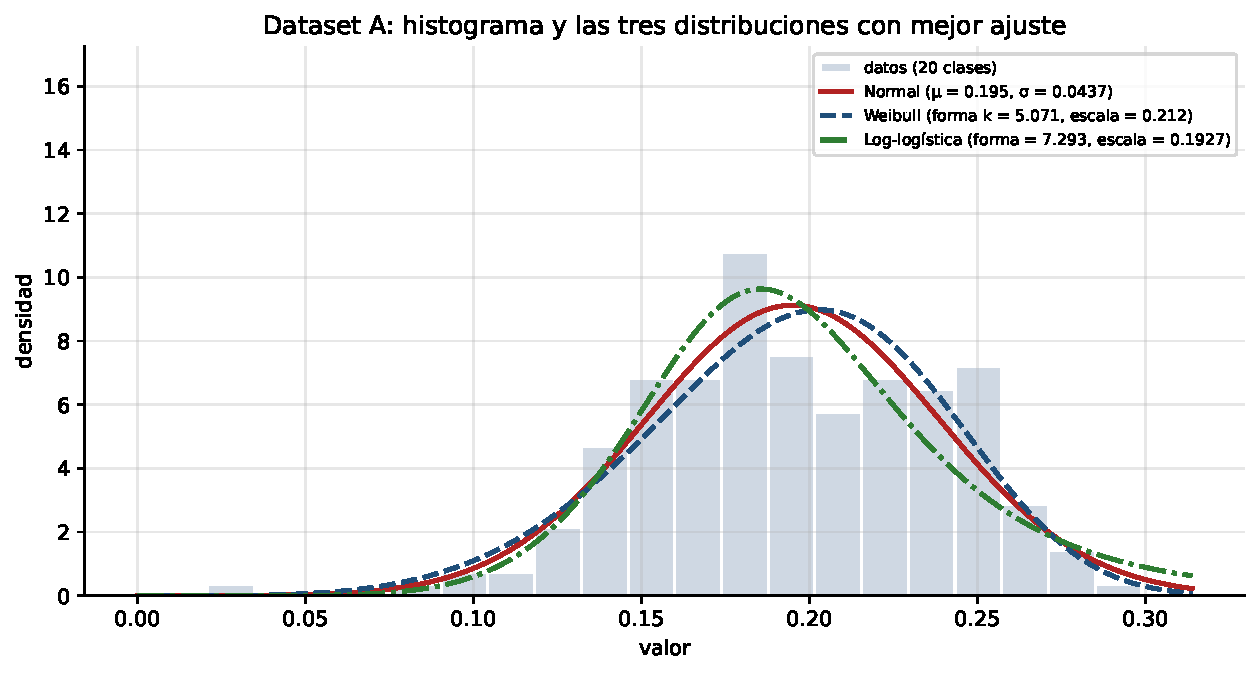
\includegraphics[width=0.82\textwidth]{figuras/53_top3_A.pdf}
\caption{Dataset A con las tres distribuciones de mejor ajuste.}
\label{fig:53A}
\end{figure}

Las tres mejores son la normal, la Weibull y la log-logística. Seleccionaría la normal con $\mu = 0{,}195$ y
$\sigma = 0{,}0437$. Tiene el menor AIC ($-680{,}59$) y el menor BIC ($-673{,}99$); la gamma consigue un SSE algo
más bajo (28,24 contra 29,15), pero por AIC y BIC queda muy atrás. La Weibull está casi empatada con la normal, a
1,2 unidades de AIC, pero la normal es más fácil de interpretar y coincide con lo que se vio en el numeral 5.1:
datos casi simétricos y concentrados alrededor de la media. El reparo habitual de la normal, que puede dar valores
negativos, aquí no pesa, porque $P(X < 0) = \Phi(-0{,}195/0{,}0437) \approx 4 \times 10^{-6}$.

Eso sí, la normal describe cada valor por separado y A está correlacionado. Si en una simulación se generan normales
independientes se pierde la dependencia, así que lo adecuado sería un modelo autorregresivo de orden 1 con esa misma
marginal, $x_t = \mu + \phi(x_{t-1} - \mu) + \varepsilon_t$, con $\phi \approx 0{,}49$ y
$\varepsilon_t \sim N(0;\ \sigma\sqrt{1 - \phi^2}) = N(0;\ 0{,}038)$.

\subsection{Dataset B}

\begin{table}[H]
\centering
\caption{Bondad de ajuste para el conjunto de datos B.}
\label{tab:53B}
\footnotesize\setlength{\tabcolsep}{4pt}
\begin{tabular}{@{}l>{\raggedright\arraybackslash}p{6.4cm}rrr@{}}
\toprule
Distribución & Parámetros & SSE & AIC & BIC \\
\midrule
\tablain{tablas/tab53_B.tex}
\bottomrule
\end{tabular}
\end{table}

\begin{figure}[H]
\centering
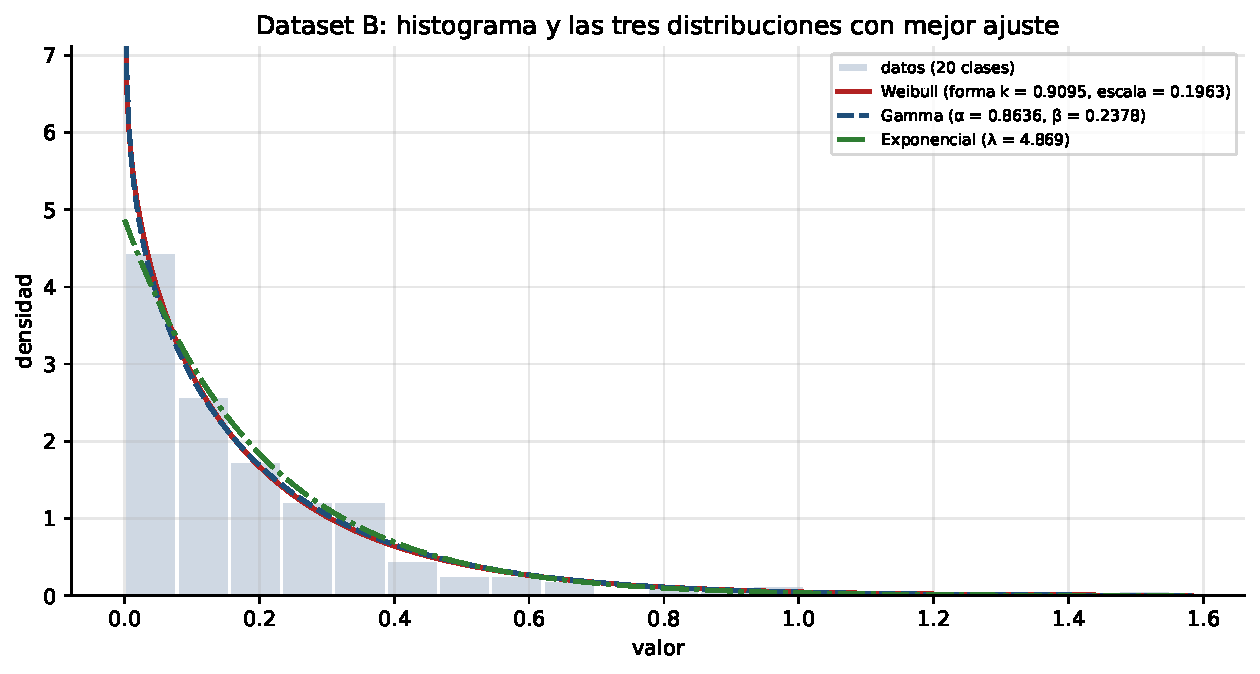
\includegraphics[width=0.82\textwidth]{figuras/53_top3_B.pdf}
\caption{Dataset B con las tres distribuciones de mejor ajuste.}
\label{fig:53B}
\end{figure}

Las tres mejores son la Weibull, la gamma y la exponencial, muy cerca entre sí. La Weibull gana en SSE y en AIC
($-232{,}26$), pero la exponencial tiene el mejor BIC ($-227{,}83$) porque usa un solo parámetro. Las formas
ajustadas de la Weibull (0,91) y de la gamma (0,86) quedan casi en 1, que es el valor con el que las dos se reducen
a la exponencial. Como la exponencial es un caso particular de ambas, se aplicó la prueba de razón de
verosimilitudes, $\Lambda = 2(\ln\hat{L}_{\text{general}} - \ln\hat{L}_{\text{exponencial}})$, con una $\chi^2$ de
un grado de libertad: frente a la gamma da $\Lambda = 2{,}97$ ($p = 0{,}085$) y frente a la Weibull
$\Lambda = 3{,}13$ ($p = 0{,}077$). El parámetro extra no mejora el ajuste de forma significativa.

Por eso seleccionaría la exponencial con $\lambda = 4{,}869$, es decir, media de 0,2054. Ajusta prácticamente igual,
tiene un solo parámetro, es la mejor según BIC y tiene una lectura directa: si B son tiempos entre llegadas, las
llegadas forman un proceso de Poisson con unas 4,9 llegadas por unidad de tiempo, lo que concuerda con el numeral 5.2.
La gaussiana inversa, en cambio, es la peor de todas (AIC de 151,99), porque B tiene valores casi nulos, como 0,0001,
y su estimador de forma se va prácticamente a cero.

\subsection{Dataset C}

\begin{table}[H]
\centering
\caption{Bondad de ajuste para el conjunto de datos C.}
\label{tab:53C}
\footnotesize\setlength{\tabcolsep}{4pt}
\begin{tabular}{@{}l>{\raggedright\arraybackslash}p{6.1cm}rrr@{}}
\toprule
Distribución & Parámetros & SSE & AIC & BIC \\
\midrule
\tablain{tablas/tab53_C.tex}
\bottomrule
\end{tabular}
\end{table}

\begin{figure}[H]
\centering
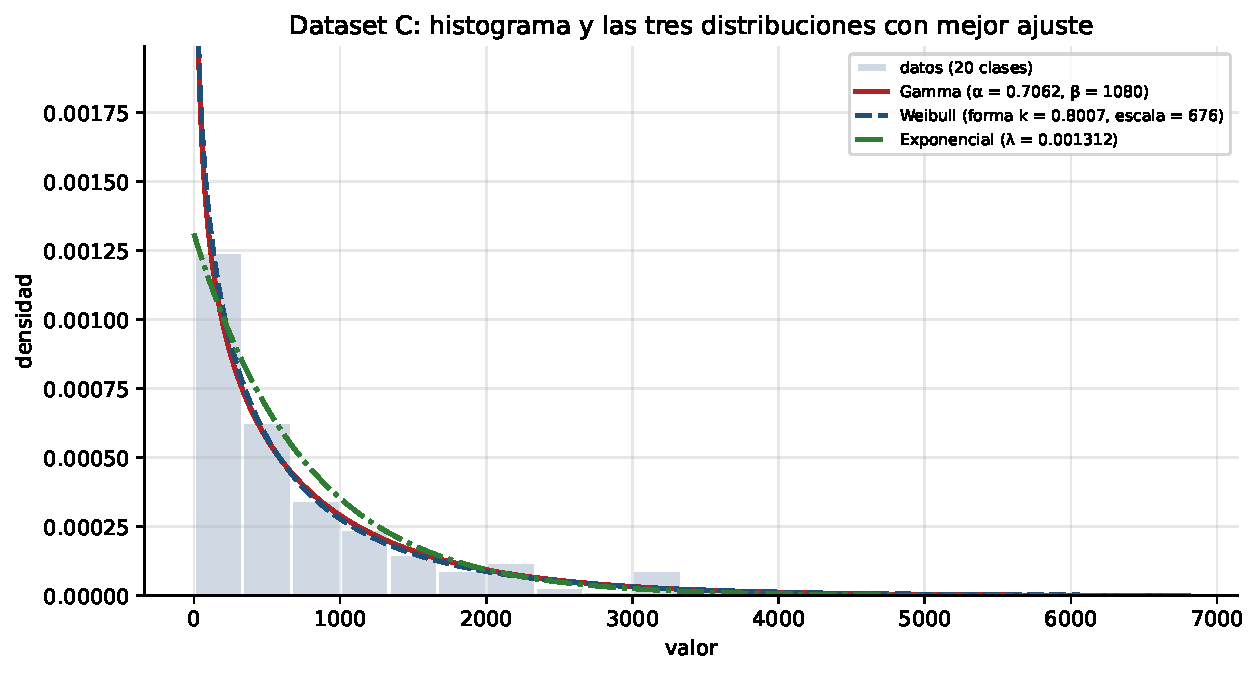
\includegraphics[width=0.82\textwidth]{figuras/53_top3_C.pdf}
\caption{Dataset C con las tres distribuciones de mejor ajuste.}
\label{fig:53C}
\end{figure}

Las tres mejores son la gamma, la Weibull y la exponencial. La gamma ($\alpha = 0{,}706$, $\beta = 1080$) tiene el
menor AIC (3040,22) y el menor BIC (3046,82), y la Weibull (forma 0,80, escala 676) le sigue a menos de una unidad de
AIC con el mejor SSE. Si hubiera que quedarse con una sola distribución, sería la gamma.

En C, sin embargo, la elección importa menos que lo encontrado en el numeral 5.2. Las dos mejores tienen forma menor
que 1, que significa más variabilidad que una exponencial, y eso es lo que resulta de mezclar exponenciales con
medias distintas. Dentro de cada quinto de la secuencia, el cociente entre la desviación estándar y la media vale
1,22, 1,33, 1,03, 0,80 y 0,95, es decir, cada tramo se parece a una exponencial, pero la media sube de 153 a 1352.
La variabilidad extra que captan la gamma y la Weibull es en buena parte el efecto de la tendencia. Para un estudio
de simulación no usaría una distribución única para C, sino tiempos exponenciales con una media que crezca a lo
largo de la secuencia.

\subsection{Dataset D}

\begin{table}[H]
\centering
\caption{Bondad de ajuste para el conjunto de datos D.}
\label{tab:53D}
\footnotesize\setlength{\tabcolsep}{4pt}
\begin{tabular}{@{}l>{\raggedright\arraybackslash}p{6.4cm}rrr@{}}
\toprule
Distribución & Parámetros & SSE & AIC & BIC \\
\midrule
\tablain{tablas/tab53_D.tex}
\bottomrule
\end{tabular}
\end{table}

\begin{figure}[H]
\centering
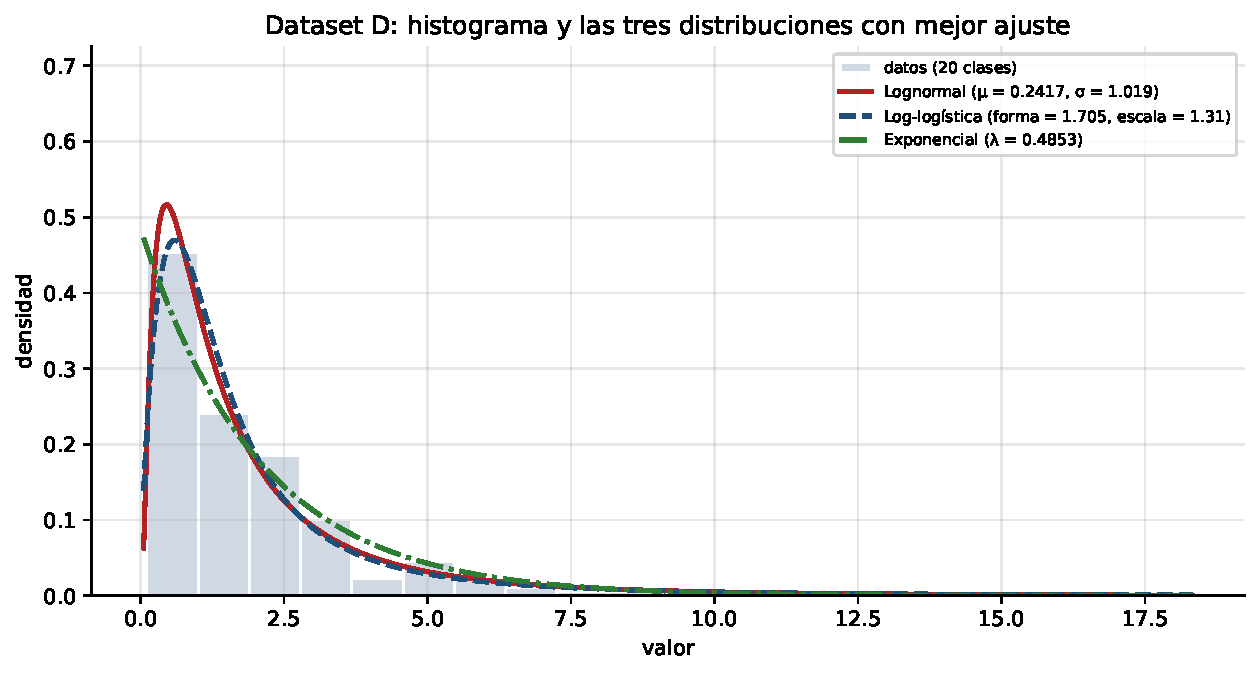
\includegraphics[width=0.82\textwidth]{figuras/53_top3_D.pdf}
\caption{Dataset D con las tres distribuciones de mejor ajuste.}
\label{fig:53D}
\end{figure}

Las tres mejores son la lognormal, la log-logística y la exponencial. Seleccionaría la lognormal con
$\mu = 0{,}2417$ y $\sigma = 1{,}019$ (parámetros del logaritmo de la variable). Tiene el menor AIC (675,89) y el
menor BIC (682,49), con 5,5 unidades de AIC de ventaja sobre la log-logística, suficiente para preferirla. La
log-logística consigue un SSE un poco menor (0,00601 contra 0,00691), pero ese criterio depende de cómo se agrupen
los datos. La lognormal además reproduce bien la muestra: su mediana es $e^{0{,}2417} = 1{,}27$ (la de los datos es
1,41) y su media, $e^{\mu + \sigma^2/2} = 2{,}14$, frente a 2,06. También encaja con el numeral 5.1, donde D mostró
una cola más pesada que la de una exponencial y un mínimo lejos de cero. La exponencial queda tercera, con un AIC 15
unidades peor.

\subsection{Resumen de la selección}

AIC y BIC eligen la misma distribución en A, C y D; en B difieren porque BIC castiga más el segundo parámetro. El
SSE es el criterio que más se aparta (gamma en A, log-logística en D), porque compara la curva con un histograma de 20
clases y su valor cambia según cómo se agrupen los datos, mientras que AIC y BIC usan los 200 valores sin agrupar.
Por eso en la selección pesaron más AIC y BIC, y el SSE sirvió para confirmar que la curva siguiera al histograma.

\begin{table}[H]
\centering
\caption{Distribución seleccionada para cada conjunto.}
\label{tab:53sel}
\small
\begin{tabular}{@{}clll@{}}
\toprule
Dataset & Distribución & Parámetros & Observación \\
\midrule
A & Normal & $\mu = 0{,}195$; $\sigma = 0{,}0437$ & Datos correlacionados: simular con AR(1) \\
B & Exponencial & $\lambda = 4{,}869$ & Weibull y gamma no la mejoran \\
C & Gamma & $\alpha = 0{,}706$; $\beta = 1080$ & No estacionario: modelar la tendencia \\
D & Lognormal & $\mu = 0{,}2417$; $\sigma = 1{,}019$ & Ventaja clara en AIC y BIC \\
\bottomrule
\end{tabular}
\end{table}

% =====================================================
\section{Conclusiones}
% =====================================================

Lo más importante que deja este laboratorio es que ajustar una distribución es el último paso del análisis de
datos de entrada, no el primero. Los cuatro conjuntos tienen el mismo tamaño y tres de ellos tienen histogramas
parecidos, pero solo B y D resultaron ser IID. Si se hubiera ido directo al ajuste, A y C habrían recibido una
distribución que describe bien su histograma y que, sin embargo, no sirve para simularlos.

Las gráficas del numeral 5.2 se complementan entre sí. La autocorrelación y el diagrama de dispersión detectaron la
dependencia de A ($r_1 = 0{,}49$), que no afecta su estabilidad; el patrón de llegadas, el conteo por intervalos y
la media móvil detectaron el cambio de nivel de C, cuya media se multiplica casi por nueve a lo largo de la
secuencia. Los indicadores numéricos (Ljung-Box y Spearman) confirmaron en cada caso lo que se veía en las gráficas.

En el ajuste, AIC y BIC fueron más confiables que el SSE para decidir, porque no dependen de cómo se agrupen los
datos. Cuando dos distribuciones quedan muy cerca conviene preferir la más simple: en B, la Weibull y la gamma ganaban
por poco, pero su forma estaba casi en 1 y la prueba de razón de verosimilitudes ($p > 0{,}07$) no justificó el
parámetro extra frente a la exponencial. En D, en cambio, la lognormal ganó con una ventaja clara.

Por último, los resultados del ajuste también ayudan a diagnosticar. Que la gamma y la Weibull de C tuvieran forma
menor que 1 era una pista de la mezcla de niveles que produce la tendencia, y lo confirmó el hecho de que cada tramo
de la secuencia, por separado, se comporte casi como una exponencial.

% =====================================================
\section{Anexos}
% =====================================================

Se adjuntan los dos cuadernos de Jupyter ejecutados, con los datos cargados y todos los resultados, además de la
carpeta con los cuatro conjuntos de datos:

\begin{itemize}[itemsep=1pt]
\item \texttt{Lab5\_5.1\_5.2\_\codigoEstudiante.ipynb}: numerales 5.1 y 5.2.
\item \texttt{Lab5\_5.3\_AjusteCurvas\_\codigoEstudiante.ipynb}: numeral 5.3.
\end{itemize}

Todas las tablas y figuras de este informe salen de esos cuadernos.

% =====================================================
\begin{thebibliography}{9}

\bibitem{banks98}
Banks, J. \emph{Handbook of Simulation: Principles, Methodology, Advances, Applications, and Practice}. John Wiley
\& Sons, Inc., 1998. Capítulo 3.

\bibitem{amat2021}
Amat Rodrigo, J. \emph{Ajuste y selección de distribuciones con Python}. Licencia CC BY-NC-SA 4.0.
\url{https://www.cienciadedatos.net/documentos/pystats01-ajuste-distribuciones-python.html}.
\url{https://doi.org/10.5281/zenodo.10006330}

\bibitem{cruz}
Cruz Roa, A. A. \emph{3. Input Data Analysis}. Diapositivas del curso Simulación Computacional, Universidad de los
Llanos.

\end{thebibliography}

\end{document}
